\section{Resultados}

\subsection{Simpson dataset}

\subsubsection{Modelos con embedding personalizado}

Los modelos descritos previamente en la sección \ref{sec:deepModels} se implementan como clasificadores para identificar cuál de los personajes principales de Los Simpson dijo un diálogo específico. En este caso se identifican como personajes principales Lisa, Bart, Homer y Marge, siendo las clases 0, 1, 2, 3 respectivamente. Se almacenan los resultados y se muestran los siguientes promedios resultados promediando.

\begin{figure}
    \centering
    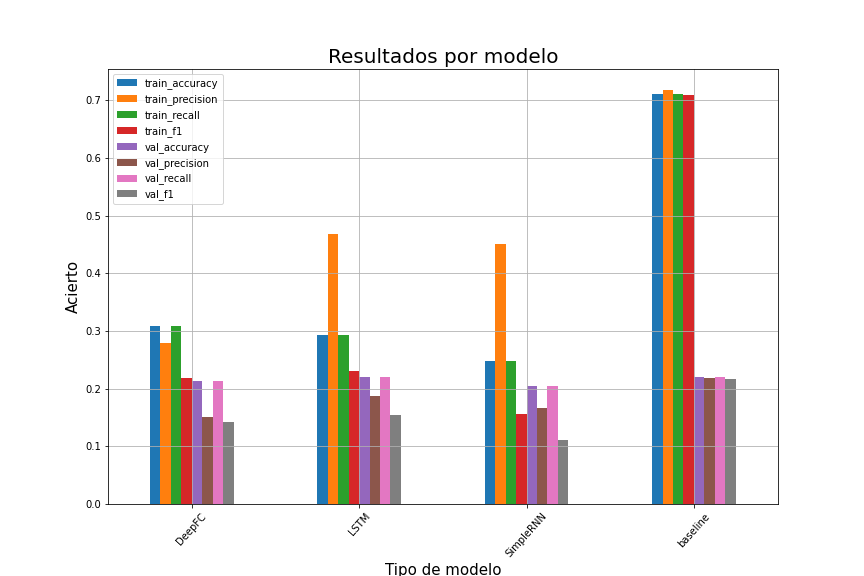
\includegraphics[width=0.9\textwidth]{results/friends/deepModels/sim_res_deep_model.png}
    \caption{Resultados por tipo de modelo}
    \label{fig:sim_deep_model}
\end{figure}

Según la figura \ref{fig:sim_deep_model}, es evidente que el modelo de tipo \textit{baseline} incurre rápidamente en \textit{overfitting}, pues su acierto en los datos de entrenamiento es muy bueno, pero en los de validación es pésimo. En cuanto a los otros modelos su rendimiento es relativamente parejo, destacando una muy buena precisión por parte de los modelos recurrentes  (LSTM y Simple RNN).\\

\begin{figure}
    \centering
    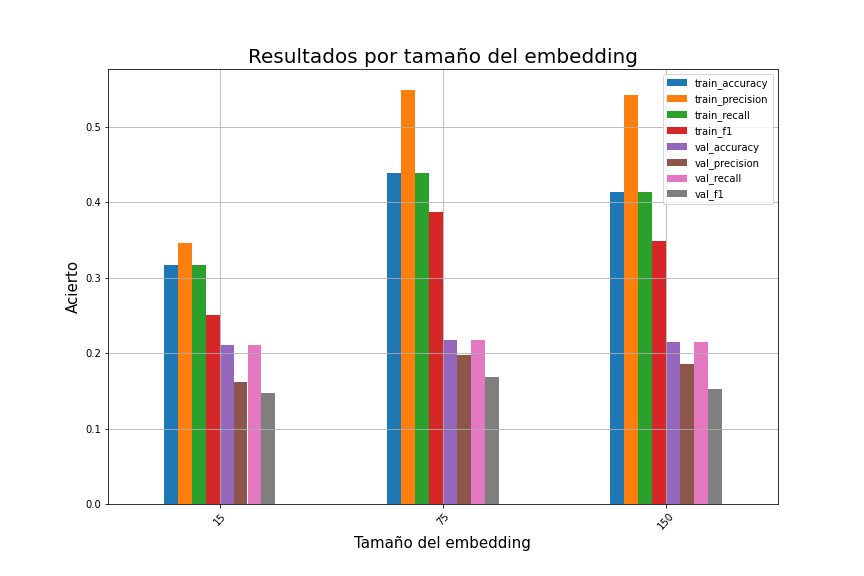
\includegraphics[width=0.9\textwidth]{results/friends/deepModels/sim_res_deep_em_size.png}
    \caption{Resultados por tamaño del embedding}
    \label{fig:sim_deep_em_size}
\end{figure}

Ahora bien, se desea comparar el efecto de los diferentes tamaños de embedding implementados, los cuales corresponden a 15, 75 y 150. Nuevamente, resulta evidente (\textit{véase fig. \ref{fig:sim_deep_em_size}}) que el embedding de tamaño 150 tiende a sobre ajustarse más a los datos de entrenamiento. No obstante, alcanza a dar un resultado ligeramente mejor que los de 15 y 75.\\

\begin{figure}
    \centering
    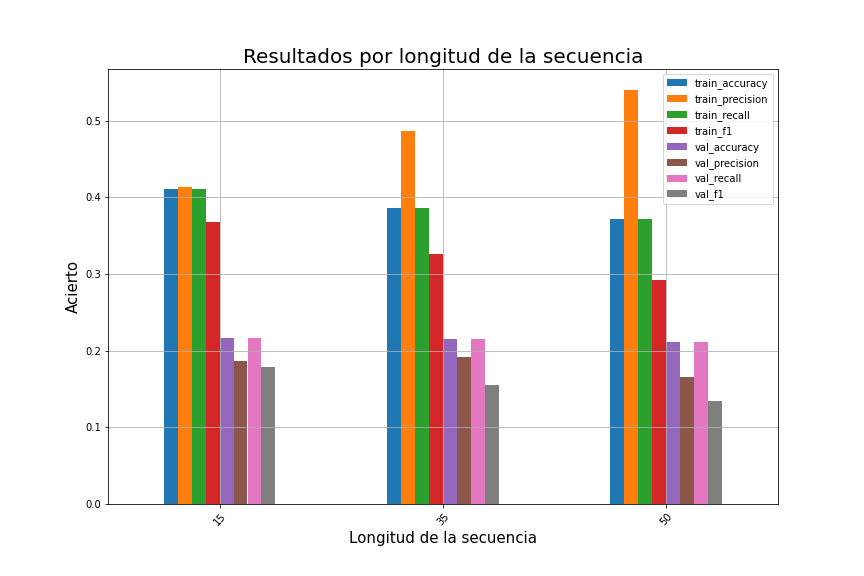
\includegraphics[width=0.9\textwidth]{results/friends/deepModels/sim_res_deep_seq_len.png}
    \caption{Resultados por el tamaño de la secuencia}
    \label{fig:sim_deep_seq_len}
\end{figure}

Finalmente, se desea comparar el efecto de utilizar secuencias de diferente tamaño (15, 35, 50). Los resultados en general son bastante similares favoreciendo un poco el f1 score de secuencias de tamaño 15.\\

Para análisis posteriores, se extrae el mejor modelo con base en el f1 score. Con este modelo se obtienen predicciones sobre datos de validación y de entrenamiento y se reentrena utilizando estos dos grupos de datos para predecir finalmente sobre los datos de test. Con base en todos estas predicciones se obtienen los siguientes resultados:

\begin{itemize}
    \item \textbf{Entrenamiento:}
    \input{results/simpson/deepModels/Test.txt}
\end{itemize}

\subsubsection{Modelos con embedding dentro de la red}

\subsubsection{Conclusiones}

\subsection{Friends dataset}

Para el caso de Friends, los modelos a implementar son exactamente los mismos. En este caso, cabe resaltar que al ser mayor cantidad de clases, se espera un resultado con desempeño más bajo. Los personajes principales en este caso son Mónica, Joey, Chandler, Phoebe, Ross y Rachel, 0, 1, 2, 3, 4, 5 respectivamente. A continuación, se muestra en consolidado de los resultados.\\

\subsubsection{Modelos con embedding personalizado}

Se puede evidenciar en la figura \ref{fig:fri_deep_model} que nuevamente el modelo \textit{baseline} incurre en \textit{overfitting} rápidamente. En este caso, cabe resaltar que los resultados de SimpleRNN no son tan parejos como los de LSTM, en especial en validación. De igual manera, DeepFC incurre en overfitting, pues sus resultados en entrenamiento mejoran, pero los de validación no se mueven.\\

\begin{figure}
    \centering
    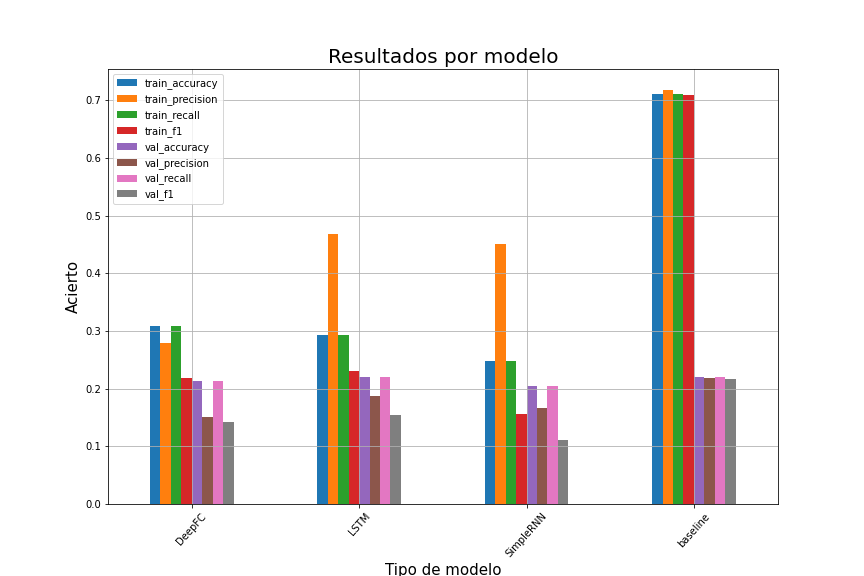
\includegraphics[width=0.9\textwidth]{results/friends/deepModels/sim_res_deep_model.png}
    \caption{Resultados por modelo}
    \label{fig:fri_deep_model}
\end{figure}

En el caso del tamaño del embedding implementado, los resultados son muy similares a los obtenidos para Los Simpson, en tanto a que a medida que se incrementa el embedding hay más posibilidad de sobre ajustar el modelo a los datos de entrenamiento.\\

\begin{figure}
    \centering
    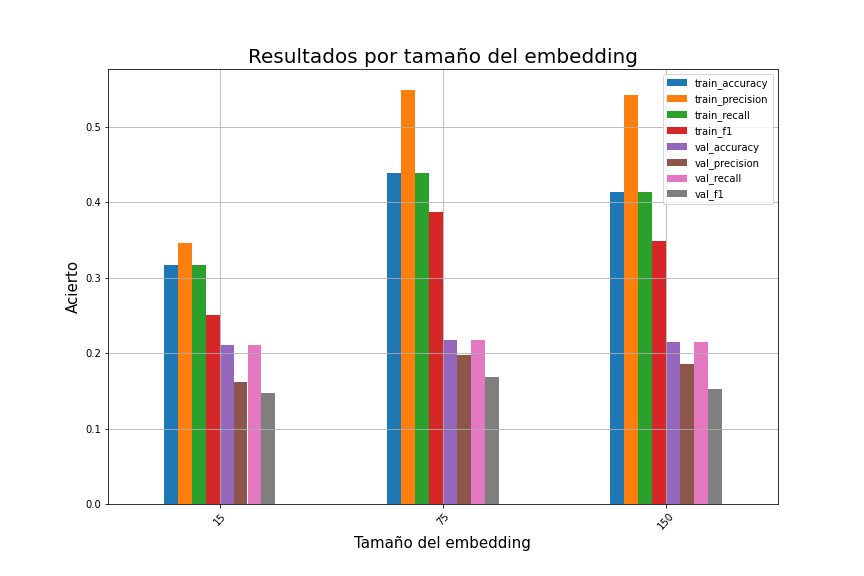
\includegraphics[width=0.9\textwidth]{results/friends/deepModels/sim_res_deep_em_size.png}
    \caption{Resultados por tamaño del embedding}
    \label{fig:fri_deep_em_size}
\end{figure}

Finalmente, en cuanto al tamaño de la secuencia, se observan resultados semejantes en validación con una pequeña diferencia en entrenamiento favoreciendo una secuencia de 15.\\

\begin{figure}
    \centering
    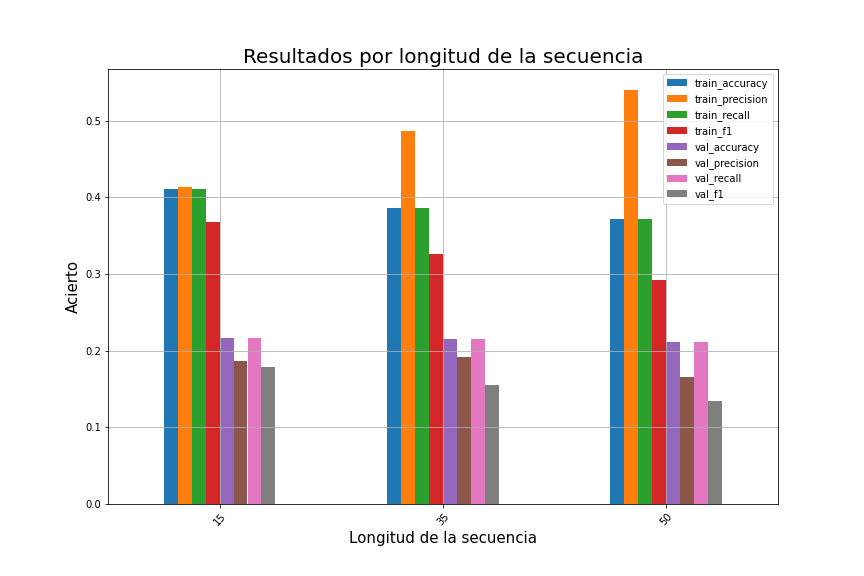
\includegraphics[width=0.9\textwidth]{results/friends/deepModels/sim_res_deep_seq_len.png}
    \caption{Resultados por tamaño de la secuencia}
    \label{fig:fri_deep_seq_len}
\end{figure}

Para análisis posteriores, se extrae el mejor modelo con base en el f1 score. Con este modelo se obtienen predicciones sobre datos de validación y de entrenamiento y se reentrena utilizando estos dos grupos de datos para predecir finalmente sobre los datos de test. Con base en todos estas predicciones se obtienen los siguientes resultados:

\begin{itemize}
    \item \textbf{Entrenamiento:}
    \input{results/friends/deepModels/Train.txt}

    \begin{figure}
        \centering
        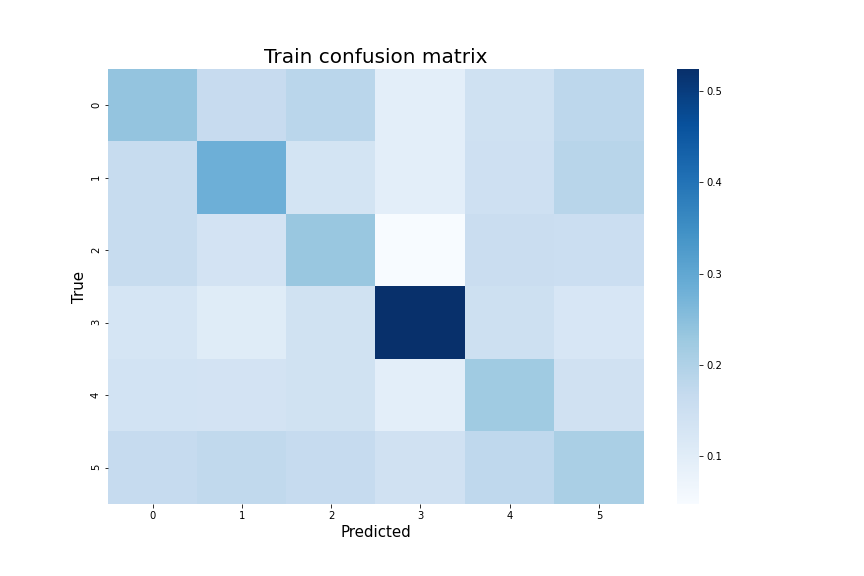
\includegraphics[width = 0.9\textwidth]{results/friends/deepModels/Train.png}
        \caption{Matriz de confusión para entrenamiento de friends}
        \label{fig:my_label}
    \end{figure}
    
    Es claro entonces que hay una clase cuya precisión es muy alta mientras que su recall es bajo (Phoebe) y por el contrario una clase cuyo recall es alto y su precisión es baja (Ross). Esto quiere decir que Para le modelo casi con total certeza identifica un guión de Ross a pesar de no ser capaz de recuperar una gran cantidad de los diálogos de él. Esto puede deberse a que es el personaje con mayor cantidad de datos. En los restantes personajes sucede que el recall es bajo, mostrando que no tiene mucha certeza en afirmar que un dialogo pertenece a un personaje en específico. En la matriz de confusión puede verse que la diagonal está ligeramente más cargada, como debería ser, pero evidentemente puede mejorar. Cabe resaltar el gran peso que tiene la predicción de la clase 3. Es por esta razón que tiene tan alta precisión pero tan bajo recall. Es como, por así decirlo, la clase por defecto.

    \item \textbf{Validación:}
    \input{results/friends/deepModels/Validation.txt}

    \begin{figure}
        \centering
        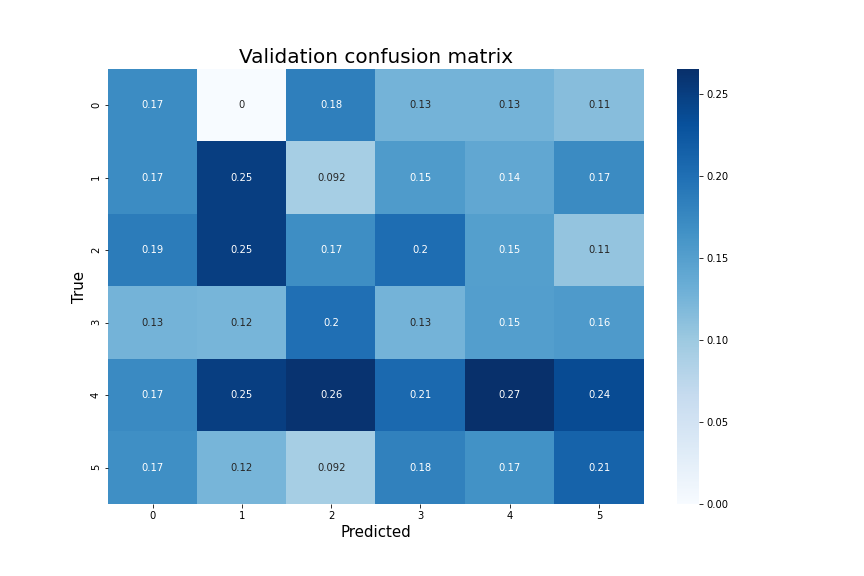
\includegraphics[width = 0.9\textwidth]{results/friends/deepModels/Validation.png}
        \caption{Matriz de confusión para validación de friends}
        \label{fig:my_label}
    \end{figure}
    
    Ahora bien, los resultados descritos previamente se repiten para el caso de validación con la diferencia que una notable disminución en la precisión de Phoebe. Nuevamente, es Ross el personaje con mayor cantidad de datos. En cuanto a la matriz de confusión, nuevamente se alcanza a rescatar que la diagonal está ligeramente más cargada. Cabe resaltar que la clase 5 tiene un desempeño bastante bajo, lo cual es evidente tanto en las métricas como en la matriz de confusión.
    
    \item \textbf{Test:}
    \input{results/friends/deepModels/Test.txt}

    \begin{figure}
        \centering
        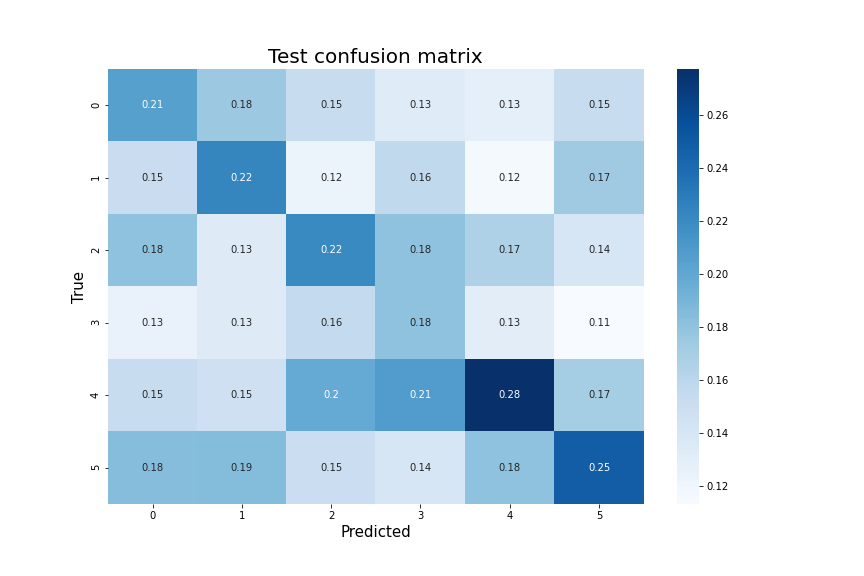
\includegraphics[width = 0.9\textwidth]{results/friends/deepModels/Test.png}
        \caption{Matriz de confusión para Test de friends}
        \label{fig:my_label}
    \end{figure}
    
    Para este caso es pertinente resaltar que, como se describió previamente, se utilizan los datos de entrenamiento y validación para entrenar nuevamente el modelo y se evalúa sobre los datos de test.

\end{itemize}



\subsubsection{Modelos con embedding dentro de la red}
\subsubsection{Conclusiones}